\subsection{Messmodell}

Der Crawler kann seine momentane Position und Ausrichtung nicht direkt messen. Es stehen jediglich vier nach vorne, hinten, links und rechts gerichtet Ultraschallsensoren zur Verfügung, die Abstandsmessungen zu den nächstliegenden Wänden vornehmen könne. Die Messwerte hängen bei einer festen Karte von der Position und Ausrichtung des Crawlers ab. 
Mit dem Messmodel wird beschrieben, welche Messergebnisse bei einem Systemzustand zu erwarten sind. Eine Messung ist Abbildung vom dreidimensionalen Zustandsraum des Laufroboters $\mathbb{S} \times \IR^2$ in einen vierdimensionalen Messraum ${\IR^+}^4$.

Da die Ultraschallsensoren des Crawler nur grobe Abstandsmessungen ermöglichen, wird ein normalverteiltes mittelwertfreies Rauschen $w_t \sim \mathcal{N}(0,\sigma)$ addiert:

\begin{align*}
\vec{z}_{t} = h(\vec{x}_t) \oplus w_t
\end{align*}

$h(x_t)$ für einen Zustand $x_t$ zu berechnen ist leicht. Es muss lediglich eine Messung auf einer virtuellen Karte an der von $x_t$ beschriebenen Position durchgeführt werden. In unserem Fall lässt sich $h$ jedoch nicht einfach invertieren. $h^{-1}$ muss nicht eindeutig sein. Die selbe Messung könnte kann in mehreren verschiedenen Zuständen beobachtet werden.
Aus $h$ lässt sich ohne weiteres die eine Likelihood $f(z_t | x_t)$ ableiten [3]. Diese beschreibt die Plausibilität einer Messung für einen gegebenen Zustand. Die Likelihood kann folgendermaßen berechnet werden $f(z_t | x_t) = f_{\mathcal{N}}(h(x_t)  - z_t)$, wobei  $f_{\mathcal{N}}$ komponentenweise in eine Normalverteilung $\mathcal{N}$ einsetzt und die resultierenden Wahrscheinlichkeiten multipliziert. Die Abbildung \ref{fig:likelihood} zeigt den Crawler in der Position im linken Bild, mit der Likelihood-Funktion für den gezeigten Zustand rechts. Der hell gelbe Punkt rechts, mit der größten Wahrscheinlichkeit befindet sich an der Stelle des Crawlers, von dem die Messung $z_t$ stammt.

\begin{figure}[ht]
	\centering
	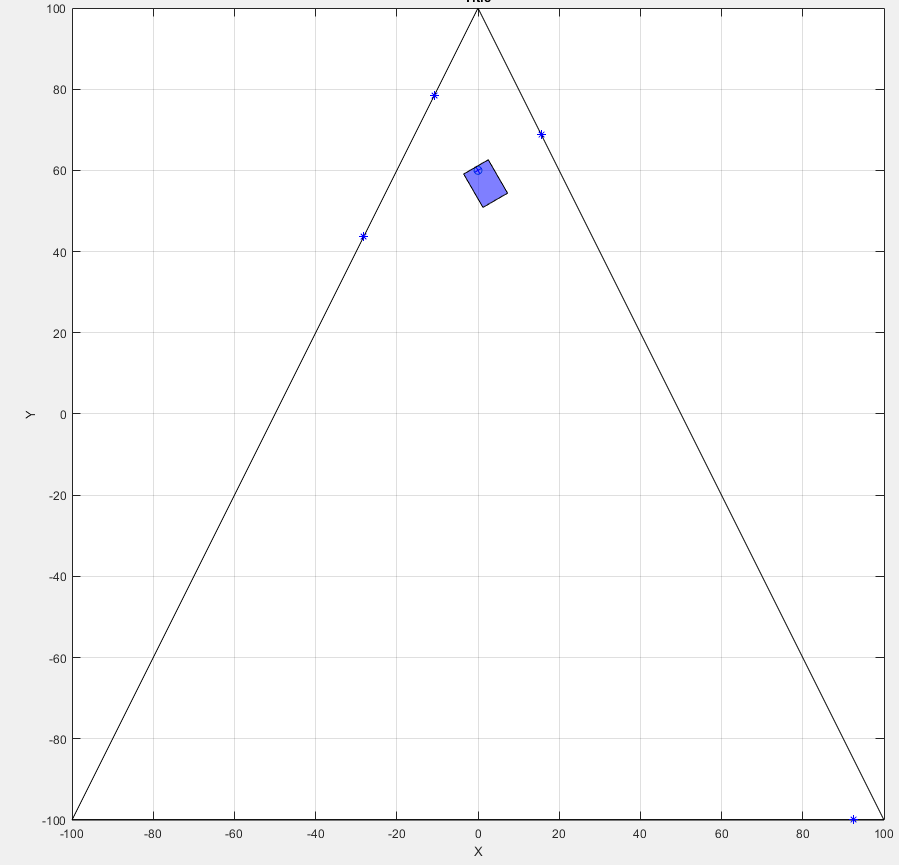
\includegraphics[width=8cm]{Images/likelihoodPosition.png}
    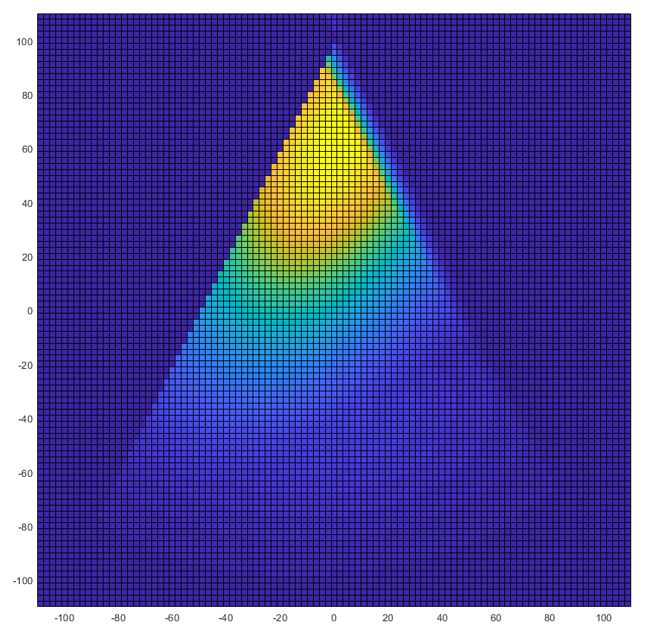
\includegraphics[width=8cm]{Images/likelihood.jpg}  
	\caption{Linkes Bild: In blau ist der Crawler auf der dreieckigen Karte eingetragen. Rechts die Likelihood-Funktion $f(z_t | x_t)$, für die Messung, die der Crawler im linken Bild aufnimmt.}
	\label{fig:likelihood}
\end{figure}
